\chapter{The Allen–Cahn PDE}
\label{ch:4}
In the previous chapter we defined the $p$--widths $\omega_p(\Omega)$ of a domain and described their variational characterisation via $p$--parameter min–max methods. A natural next step is to seek numerical approximations to $p$--width–realising hypersurfaces. While direct hypersurface sweep–outs are conceptually straightforward, their numerical implementation is complicated by the need to manage topological changes. In this chapter we present an alternative approach based on the Allen--Cahn PDE, following the 2018 paper of my supervisor, Guaraco~\cite{Guaraco18}. This PDE-based variational framework connects min--max critical points of a scalar energy to minimal hypersurfaces via their zero--level set and offers a flexible setting in which topology changes occur naturally. We will develop the finite element methods needed to apply this framework in practice and use them to explore $p$--widths for a range of domains.

\noindent We recall the \emph{Allen–Cahn equation}
\begin{equation}\label{eq:allen-cahn-pde}
    -\varepsilon\Delta u+\frac{1}{\varepsilon}W'(u)=0 \quad \text{in } \Omega,
\end{equation}
where $W\colon\mathbb{R}\to[0,\infty)$ is a \emph{double–well potential} with precisely two non-degenerate global minima, say at $\pm1$ with $W''(\pm1)>0$. A canonical example, used throughout this work, is
\begin{align*}
W(u) = \frac14(1-u^2)^2.
\end{align*}

\noindent In the mountain pass dictionary, the elements are:
\begin{itemize}
    \item \textbf{Space of functions:} the Sobolev space $H^1(\Omega)$.
    \item \textbf{Admissible families:} smooth $p$–parameter families $\Phi \colon Y \to H^1(\Omega)$.
    \item \textbf{Functional:} the Allen–Cahn energy
    \begin{equation}\label{eq:allen-cahn-energy}
      E_\varepsilon(u) = \int_{\Omega} \frac{\varepsilon}{2}|\nabla u|^{2} + \frac{1}{\varepsilon} W(u) \,\mathrm{d}x, \qquad u\in H^{1}(\Omega).
    \end{equation}
    \item \textbf{Mountains:} the $p$–parameter min–max levels of $E_\varepsilon$
    \begin{equation}\label{eq:minmax-level}
        c_{\varepsilon}^{(p)} = \inf_{\Phi} \ \sup_{y \in Y} E_{\varepsilon}(\Phi(y)),
    \end{equation}
    where the infimum is over all $p$–parameter families $\Phi$ in the admissible class $Y$.
\end{itemize}

\noindent Guaraco's theorem shows that, as $\varepsilon \to 0$,
\begin{align*}
\frac{1}{2\sigma} \, c_{\varepsilon}^{(p)} \ \longrightarrow \ \omega_p(\Omega),
\quad \text{where } 
\sigma = \int_{-1}^1 \sqrt{2 W(s)} \,\mathrm{d}s,
\end{align*}
\noindent and the zero level--sets $\{u_{\varepsilon}=0\}$ of the associated min–max solutions converge (in the varifold sense) to a stationary hypersurface $\Gamma$ realising $\omega_p(\Omega)$. In dimensions $n \leq 7$, $\Gamma$ is a smooth embedded minimal hypersurface (possibly with multiplicity).

\noindent Thus, the Allen–Cahn PDE offers a PDE–based realisation of the geometric widths of Chapter (\ref{ch:3}) and a computationally tractable route to approximating them. This formulation has a key advantage over direct hypersurface sweep–outs, which is that \emph{topology change} is effortless. In a geometric sweep–out one must prescribe how slices split or merge, a delicate and non–local combinatorial task. In the function–space setting, the zero level--set $\{u=0\}$ can break, merge, or change topology continuously as $u$ varies, with no extra bookkeeping - making implementation much simpler. This flexibility is one of the main reasons the Allen–Cahn framework is so powerful for constructing $p$–width–realising hypersurfaces.

\noindent The numerical study of \eqref{eq:allen-cahn-pde} presented in the remainder of this chapter builds on this viewpoint, and is revisited in the \emph{Further Directions} chapter (\ref{ch:5}) as a potential framework for testing conjectures on widths in various domains, including Conjecture (\ref{conjecture1}).

\section{Deriving the Allen–Cahn PDE from the Energy}

We now verify that \eqref{eq:allen-cahn-pde} is indeed the Euler–Lagrange equation associated to the energy \eqref{eq:allen-cahn-energy}. Let $0 < \varepsilon \ll 1$, and let $v\in H^{1}(\Omega)$ be an arbitrary test function consistent with the chosen boundary conditions (for example, $v|_{\partial\Omega}=0$ in the Dirichlet case). The \emph{first variation} of $E_\varepsilon$ in the direction $v$ is
\begin{align*}
  \big\langle E_\varepsilon'(u),\,v \big\rangle
  &= \frac{\mathrm d}{\mathrm dt} E_\varepsilon(u+tv)\bigg|_{t=0} \\
  &= \int_{\Omega} \varepsilon \nabla u\cdot\nabla v-\frac{1}{\varepsilon} W'(u) \, v \ \mathrm dx.
\end{align*}
If $v$ vanishes on $\partial\Omega$, integration by parts in the first term yields
\begin{align*}
  \big\langle E_\varepsilon'(u),\,v \big\rangle
  &= \int_{\Omega} \left(-\varepsilon \Delta u-\frac{1}{\varepsilon} W'(u) \right) v \ \mathrm dx.
\end{align*}
A critical point of $E_\varepsilon$ satisfies $\langle E_\varepsilon'(u),v\rangle=0$ for all such $v\in H^1(\Omega)$. By the fundamental lemma of the calculus of variations, this is equivalent (in the weak sense) to the Euler–Lagrange equation \eqref{eq:allen-cahn-pde}. In other words, the Allen–Cahn PDE is precisely the stationarity condition for its associated energy functional.

\section{Allen–Cahn Energy, Perimeter Limit, and p–Widths}\label{sec:Modica-Mortola}

\noindent
A key fact underlying the connection between the Allen--Cahn min--max levels and geometric $p$--widths is that the Allen--Cahn energy (\ref{eq:allen-cahn-energy}) is a \emph{diffuse–interface approximation} to the length (in $2$--d) or area (in higher dimensions) of an interface. In the $\varepsilon \to 0$ limit, this diffuse description collapses onto a \emph{sharp interface} $\Gamma$ which is a minimal hypersurface in the appropriate variational sense.

\begin{theorem}[The Modica–Mortola Theorem, \cite{Modica77}]
Let $\sigma = \int_{-1}^1 \sqrt{2W(s)}\,ds$. As $\varepsilon \to 0$, the functionals $E_\varepsilon$ $\Gamma$–converge in $L^1(\Omega)$ to the perimeter functional,
\begin{align*}
E_\varepsilon \ \xrightarrow{\Gamma}\  2\sigma\ \mathrm{Per}(\cdot).
\end{align*}
We say that $E_{\varepsilon}$ $\Gamma$-converges to $E$ on $X$ as $\varepsilon\to 0$ if the following two conditions hold,
\begin{itemize}
    \item (\emph{Lower bound})  
    If $u_\varepsilon \to u$ in $L^1$, then
    \begin{align*}
    \liminf_{\varepsilon \to 0} E_\varepsilon(u_\varepsilon) \ \ge\  2\sigma\ \mathrm{Per}(\{u=1\}).
    \end{align*}
    \item (\emph{Recovery sequence})  For every set $E$ of finite perimeter, there exist $u_\varepsilon$ with $u_\varepsilon \to \chi_E - \chi_{\Omega\setminus E}$ in $L^1$ and
    \begin{align*}
    \lim_{\varepsilon \to 0} E_\varepsilon(u_\varepsilon) =  2\sigma\ \mathrm{Per}(E).
    \end{align*}
\end{itemize}
Where $\mathrm{Per}(E)$ is the perimeter of $E$, i.e.~the length/area of $\partial E$ in the sense of De Giorgi (equivalently, the relative perimeter in $\Omega$).
\end{theorem}

\noindent
\textbf{Heuristic picture.}
In one dimension, the optimal profile connecting $-1$ and $+1$ solves
\begin{align*}
    q'(t) = \sqrt{2W(q(t))}, \quad q(-\infty)=-1,\ q(+\infty)=+1,
\end{align*}
and has a fixed energy cost $2\sigma$ independent of scale.\\
\noindent In higher dimensions, near a smooth interface $\Gamma$ the optimal phase field is $u(x) \approx q\big(d(x,\Gamma)/\varepsilon\big)$, where $d(\cdot,\Gamma)$ is signed distance to $\Gamma$. \\
\noindent Integrating the one–dimensional profile across $\Gamma$ shows that the total energy is
\begin{align*}
E_\varepsilon(u) \ \approx\  2\sigma\,\mathcal{H}^{n-1}(\Gamma) + o(1),
\end{align*}
so $E_\varepsilon$ concentrates in an $O(\varepsilon)$–thick layer around $\Gamma$.

\noindent
\textbf{From minimal surfaces to unstable minimal surfaces.}
\begin{itemize}
    \item For \emph{minimisers} of $E_\varepsilon$, Modica--Mortola implies that the zero level--set tends to a \emph{stable} minimal hypersurface that minimises perimeter given the boundary data. For this reason the first numerical implementation that we made, in Section (\ref{sec:minimal-surfaces-program}), was a surface evolver that created a triangulated mesh, approximating a 3-$d$ surface and performed gradient descent on the area of the triangles with respect to its vertices, iteratively and visualises the minimal surface it converges to.
    \item Guaraco’s insight was to run a \emph{$p$--parameter min--max} in the function space $H^1(\Omega)$. The $p$--th min--max value $c_\varepsilon^{(p)}$ then approximates $2\sigma$ times the smallest maximal area achievable by any admissible $p$--sweep--out of functions, and by the definition of $p$--widths this is exactly $2\sigma\,\omega_p(\Omega)$. In the limit,
    \begin{align*}
        \frac{1}{2\sigma} c_\varepsilon^{(p)} \to \omega_p(\Omega),
    \end{align*}
    and the zero level--sets of the corresponding solutions converge to a stationary hypersurface realising $\omega_p(\Omega)$. Unlike the minimiser case, this hypersurface is an \emph{unstable} minimal surface - the PDE framework produces precisely the unstable minimal hypersurfaces predicted by Almgren–Pitts min–max theory. This was the basis for our second implementation in Section (\ref{sec:planar-widths-program}).
\end{itemize} 

\begin{figure}[ht]
    \centering

    % Panel A: Double–well potential & optimal 1D profile
    \begin{tikzpicture}
  % Title
  \node[anchor=west] at (1,3.5)
    {\small \textbf{(Top) Double--well $W$ and optimal 1D transition $q$}};

  \begin{groupplot}[
      group style={
        group size=2 by 1,
        horizontal sep=2.5cm, % space between the two plots
        y descriptions at=edge left
      },
      width=6.7cm, height=4.1cm,
      every axis plot/.append style={thick}
  ]

    % Left plot: W(u)
    \nextgroupplot[
      xmin=-1.4, xmax=1.4, ymin=-0.02, ymax=0.35,
      axis lines=left,
      xlabel={$u$}, ylabel={$W(u)$},
      xtick={-1,0,1}, ytick={0,0.25},
      samples=200,
      domain=-1.2:1.2
    ]
      \addplot {(1 - x^2)^2/4};
      \addplot[densely dashed] coordinates {(-1,0) (-1,0.001)};
      \addplot[densely dashed] coordinates {(1,0) (1,0.001)};
      \node[below] at (axis cs:-1,0) {$-1$};
      \node[below] at (axis cs:1,0) {$1$};

    % Right plot: q(t)
    \nextgroupplot[
      xmin=-3.2, xmax=3.2, ymin=-1.2, ymax=1.2,
      axis lines=left,
      xlabel={$t$}, ylabel={$q(t)$},
      xtick={-3,0,3}, ytick={-1,0,1},
      samples=200,
      domain=-3:3
    ]
      \addplot {tanh(x/1.41421356237)};
      \addplot[densely dashed] coordinates {(-3,-1) (3,-1)};
      \addplot[densely dashed] coordinates {(-3,1) (3,1)};
      \node[right] at (axis cs:3,-1) {$-1$};
      \node[right] at (axis cs:3,-1) {$-1$};

  \end{groupplot}
\end{tikzpicture}

    \vspace{0.8em}

    % Panel B: Diffuse interface for finite epsilon
    \begin{tikzpicture}[scale=1]
  % Title
  \node[anchor=west] at (-6.1,3.0) {\small \textbf{(Middle) Diffuse interface of thickness $\varepsilon$ around a curve $\Gamma$}};

  % Domain rectangle
  \draw[thick] (-6, -2) rectangle (6, 2);

  % A wavy curve Gamma
  \draw[name path=Gamma, ultra thick] (-5.5,0.4) .. controls (-3,1.1) and (-1,-0.8) .. (1,0.3)
                                      .. controls (2,0.8) and (3.5,-0.2) .. (5.5,0.6);
  \node[above right] at (1.05,0.45) {$\Gamma$};

  % Build an "interface tube" of thickness ~ epsilon around Gamma
  % We'll approximate the offset by drawing a second wavy line and filling between.
  \path[name path=GammaUp] (-5.5,0.7) .. controls (-3,1.4) and (-1,-0.5) .. (1,0.6)
                           .. controls (2,1.1) and (3.5,0.1) .. (5.5,0.9);
  \path[name path=GammaDn] (-5.5,0.1) .. controls (-3,0.8) and (-1,-1.1) .. (1,0.0)
                           .. controls (2,0.5) and (3.5,-0.5) .. (5.5,0.3);

  % Fill the band (transition layer)
  \tikzfillbetween[of=GammaUp and GammaDn]{gray,opacity=0.25};

  % Labels for phases
  \node at (-4.8,1.6) {$u \approx +1$};
  \node at (4.8,-1.6) {$u \approx -1$};

  % Bracket to show thickness ~ epsilon
  \draw[<->,>=Latex] (-2.8,1.15) -- (-2.8,0.45);
  \node[right] at (-2.8,0.8) {$\sim \varepsilon$};
\end{tikzpicture}

    \vspace{0.8em}

    % Panel C: Sharp interface limit
    \begin{tikzpicture}[scale=1]
  % Title
  \node[anchor=west] at (-6.1,3.0) {\small \textbf{(Bottom) As $\varepsilon \downarrow 0$, the layer shrinks and energy concentrates on $\Gamma$}};

  % Domain rectangle
  \draw[thick] (-6, -2) rectangle (6, 2);

  % The same Gamma curve
  \draw[name path=Gamma2, ultra thick] (-5.5,0.4) .. controls (-3,1.1) and (-1,-0.8) .. (1,0.3)
                                       .. controls (2,0.8) and (3.5,-0.2) .. (5.5,0.6);

  % A thinner band to represent smaller epsilon
  \path[name path=GammaUp2] (-5.5,0.55) .. controls (-3,1.25) and (-1,-0.65) .. (1,0.45)
                            .. controls (2,0.95) and (3.5,-0.05) .. (5.5,0.75);
  \path[name path=GammaDn2] (-5.5,0.25) .. controls (-3,0.95) and (-1,-0.95) .. (1,0.15)
                            .. controls (2,0.65) and (3.5,-0.35) .. (5.5,0.45);

  \tikzfillbetween[of=GammaUp2 and GammaDn2]{gray,opacity=0.18};

  % Energy concentration markers (short normal spikes on Gamma) 
  \foreach \x/\y/\dx/\dy in {
    -4.8/0.55/0.0/0.4, -3.6/0.95/0.0/0.35, -2.4/0.25/0.0/0.35,
    -1.2/-0.35/0.0/0.35, 0.0/0.25/0.0/0.35, 1.2/0.45/0.0/0.35,
    2.7/0.45/0.0/0.35, 4.2/0.35/0.0/0.35
  }{
    \draw[line width=0.4pt,opacity=0.5] (\x,\y) -- ++(0,0.22);
  }

  % Label
  \node[above right] at (1.2,0.5) {$\Gamma$};
  \node at (4,1.6) {$\text{energy} \;\propto\; \delta_{\Gamma}$ as $\varepsilon\!\downarrow\!0$};
\end{tikzpicture}

    \caption{Top: the double–well potential $W$ and the optimal 1D transition $q$ (energy cost $2\sigma$).  
    Middle: for small $\varepsilon$, a diffuse interface of thickness $\sim \varepsilon$ forms around a curve $\Gamma$.  
    Bottom: as $\varepsilon \to 0$, the transition layer shrinks and the energy localises on $\Gamma$, recovering $2\sigma\times \mathrm{Length}(\Gamma)$ (or area in higher dimensions).}
    \label{fig:AC-interface-diagram}
\end{figure}
\FloatBarrier

\section{Numerical Implementations}
The first stage of this project focused on developing the numerical methods described in this section. We began with the area functional, chosen as a simpler starting point than the Allen–Cahn energy due to its clear geometric interpretation. Using this, I built a finite element method (FEM)–based visualisation tool capable of evolving surfaces towards minimal surfaces. We then outline the algorithm - implemented by my supervisor - for extending this framework to unstable minimal surfaces via a mountain–pass method.  
\noindent Building on this foundation, we investigated how the same program could be adapted to study min--max points of the Allen–Cahn energy. I implemented FEM-based methods for computing this energy over triangulated domains, as well as for evaluating its gradient and Hessian efficiently by exploiting the expected sparsity of the Hessian matrix. My supervisor subsequently developed an interactive application that enables users to load triangulated domains, apply these methods to evolve surfaces with respect to the Allen–Cahn energy, and visualise the resulting level sets - aiming to detect widths, as anticipated by his 2018 work (\cite{Guaraco18}).

\subsection{Finite Element Method for the Area Functional}\label{sec:minimal-surfaces-program}
We begin by considering the area functional as a simpler starting point than the Allen–Cahn energy, owing to its direct geometric interpretation. Our aim is to develop a numerical framework capable of evolving surfaces towards minimal surfaces by optimising the \emph{area functional} over the vertex coordinates of a fixed-topology triangulated surface. This approach complements the Allen–Cahn method by working directly in $\mathbb{R}^3$ with the mesh geometry.

\noindent We store the \emph{topology} and \emph{geometry} separately, methods for handling this were based on the course notes of the Finite Element module at Imperial, \cite{FEMnotes}, and a book on FEM theory, \cite{Ern04}:
\begin{itemize}
    \item \textbf{ASurf} (\emph{Abstract surface}): a $3\times F$ integer matrix where each column $(i,j,k)$ lists the vertex indices of a face.
    \item \textbf{VCoord} (\emph{Vertex coordinates}): a $3\times N$ real matrix where each column $v_\ell = (x_\ell, y_\ell, z_\ell)$ is the position of vertex $\ell$ in $\mathbb{R}^3$.
\end{itemize}
This separation allows the same topology to be reused for multiple geometric configurations.

\noindent Given a face $(i,j,k)$ with vertices $v_i, v_j, v_k \in \mathbb{R}^3$, we compute its area as
\[
\operatorname{Area}(v_i,v_j,v_k)
= \frac12 \sqrt{\det G},
\quad
G =
\begin{pmatrix}
p\cdot p & p\cdot q \\
p\cdot q & q\cdot q
\end{pmatrix},
\]
where $p = v_j - v_i$, $q = v_k - v_i$. The discrete area functional is then the sum of the area over all the faces in the mesh,
\[
\mathcal{A}(V) = \sum_{(i,j,k) \in \mathrm{ASurf}} \operatorname{Area}(v_i,v_j,v_k),
\]
which we view as a smooth function of each vertex
\[
\mathcal{A} : \mathbb{R}^{3N} \to \mathbb{R}.
\]
A \emph{discrete minimal surface} is then any $V$ with $\nabla \mathcal{A}(V) = 0$, with saddle points corresponding to unstable minimal surfaces. The gradient of the total area wrt. each vertex $v_i$, $\nabla_{v_i} \mathcal{A} \in \mathbb{R}^3$, is obtained by summing contributions from all incident faces:
\[
\nabla_{v_i} \operatorname{Area}(v_i,v_j,v_k)
= 2||v_k - v_i||^2v_i - 2\langle v_k-v_i, v_k-v_j\rangle v_j + 2\langle v_j-v_i, v_k-v_i \rangle v_k,
\]
homogeneous in all arguments. We then can evolve free (non-boundary) vertices with respect to the discrete area functional using the standard gradient descent iteration,
\[
V^{i+1} = V^i - \alpha \nabla \mathcal{A}(V^i),
\]
with fixed step size $\alpha$ and for a given number of iterations - both chosen by the user in my program. The user can then view the evolved surface and perform more evolutions.

\noindent We have an additional evolution method that adds a velocity term $M^i$ that is used in the gradient descent with momentum iteration,
\[
M^{i+1} = \beta M^i - \alpha \nabla \mathcal{A}(V^i),
\quad
V^{i+1} = V^i + M^{i+1},
\]
with $\beta \in (0,1)$ chosen by the user as well as the same parameters in the standard gradient descent. This method can accelerate convergence in the highly non--convex (discrete) surface space, especially in shallow valleys.

\noindent The FEM-based gradient descent converges to a stable minimal surface under the given boundary conditions. The figure below shows an example obtained from a triangulated cylindrical mesh, illustrating the method’s convergence behaviour.

\begin{figure}[ht]
  \centering
  \begin{subfigure}{0.49\textwidth}
    \centering
    \includegraphics[width=\linewidth]{figures/img1.png}
    \caption{Triangulated mesh of a cylinder before gradient descent evolution.}
    \label{fig:ac-gd-a}
  \end{subfigure}\hfill
  \begin{subfigure}{0.49\textwidth}
    \centering
    \includegraphics[width=\linewidth]{figures/img2.png}
    \caption{Evolved surface that has converged to a stable catenoid.}
    \label{fig:ac-gd-b}
  \end{subfigure}
  \caption{Minimal surface produced by FEM-based gradient descent of the discrete area functional, starting from a triangulated cylindrical mesh (left). The final configuration illustrates convergence to a stable minimal surface under the given boundary constraints (right).}
  \label{fig:ac-gd-side-by-side}
\end{figure}
\FloatBarrier
\noindent This framework provides the foundation for computing unstable minimal surfaces via the mountain–pass algorithm, and for adapting the same approach to the Allen–Cahn energy in the next subsection. And, as previously mentioned, my supervisor then implemented a comprehensive version of this application for finding unstable minimal surfaces. The algorithm behind this is outlined below.

\noindent\textbf{Mountain–pass search for unstable minimal surfaces.}\\
To find index--1 saddles of $\mathcal{A}$:
\begin{enumerate}
    \item Choose two low–area configurations $V^-$ and $V^+$ in different basins.
    \item Interpolate vertex positions to get a path $\gamma(t)$.
    \item Find $t^\star$ maximising $\mathcal{A}(\gamma(t))$.
    \item Perform gradient descent orthogonal to the path tangent at $t^\star$.
    \item Update the path and repeat until the peak energy converges.
\end{enumerate}

\noindent\textbf{Implementation notes}
\begin{itemize}
    \item \textbf{Precomputation:} store face adjacencies and edge vectors for fast gradient assembly.
    \item \textbf{Boundary constraints:} fix coordinates of boundary vertices throughout iterations.
    \item \textbf{Contributions:} I implemented the program for finding minimal surfaces and my supervisor implemented a comprehensive program for also finding unstable minimal surfaces.
\end{itemize}

\subsection{Finite Element Method for the Allen--Cahn Energy}\label{sec:planar-widths-program}
Having established a finite element framework for evolving surfaces with respect to the area functional, we now turn to the Allen--Cahn energy as a tool for studying $p$–widths. In my supervisor's approach~\cite{Guaraco18}, the Allen-Cahn equation provides a PDE-based variational framework whose min--max critical points correspond, via the volume (or length in the planar case) of their zero level--set, to approximations of the $p$--widths. Our goal in this section is therefore not only to adapt the FEM framework developed earlier to this energy, but to use it as a numerical engine for approximating $p$–width–realising hypersurfaces and visualising them in triangulated domains.

\noindent To carry out the finite element discretisation of the Allen–Cahn energy, we approximate the solution $u \in H^{1}(\Omega)$ using continuous, piecewise–linear ($P_{1}$) basis functions defined over a conforming triangulation $\mathcal{T}_{h}$ of the domain. Each basis function is associated with a mesh vertex and takes the value $1$ at its own vertex and $0$ at all others, varying linearly within each element. The figure below illustrates three such basis functions on the reference triangle, which together span the space $P_{1}(T)$ for a single element.

\begin{figure}[ht]
    \centering
    \begin{subfigure}{0.32\textwidth}
        \centering
        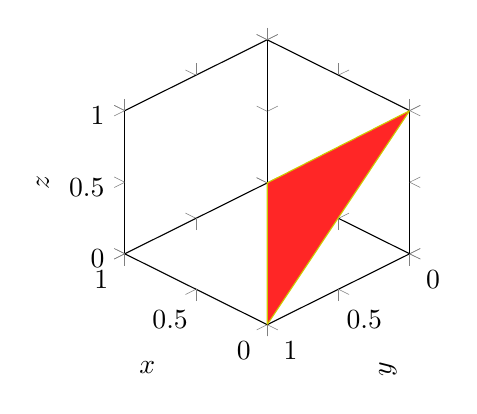
\begin{tikzpicture}
\begin{axis}[
  view={-135}{35},
  width=5.2cm, height=5.2cm,
  xlabel={$x$}, ylabel={$y$}, zlabel={$z$},
  xmin=0, xmax=1, ymin=0, ymax=1, zmin=0, zmax=1,
  axis lines=box, tick align=outside
]
\addplot3[
  patch, patch type=triangle,
  fill=red!85, draw=black
] coordinates {
  (0,0,1)
  (0,1,0)
  (1,0,0)
};
\end{axis}
\end{tikzpicture}
 % include the first plot
        \caption{First basis function}
        \label{fig:red}
    \end{subfigure}
    \begin{subfigure}{0.32\textwidth}
        \centering
        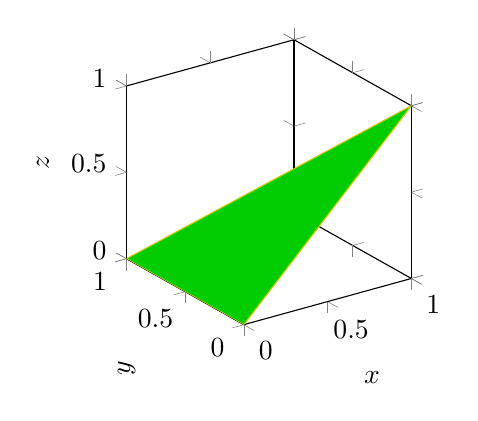
\begin{tikzpicture}
\begin{axis}[
  view={-35}{25},
  width=5.2cm, height=5.2cm,
  xlabel={$x$}, ylabel={$y$}, zlabel={$z$},
  xmin=0, xmax=1, ymin=0, ymax=1, zmin=0, zmax=1,
  axis lines=box, tick align=outside
]
\addplot3[
  patch, patch type=triangle,
  fill=green!80!black, draw=black
] coordinates {
  (1,0,1)
  (0,1,0)
  (0,0,0)
};
\end{axis}
\end{tikzpicture}
 % include the second plot
        \caption{Second basis function}
        \label{fig:green}
    \end{subfigure}
    \begin{subfigure}{0.32\textwidth}
        \centering
        \input{figures/p1_3.tex} % include the third plot
        \caption{Third basis function}
        \label{fig:blue}
    \end{subfigure}
    \caption{The three triangular basis functions plotted on the reference element.}
    \label{fig:three-basis}
\end{figure}

\noindent With these basis functions $\{\phi_i\}_{i=1}^N$ defined, we can express the finite element approximation $u_h$ of $u$ as a linear combination of them,
\[
u_{h}(x) = \sum_{i=1}^{N} U_{i} \, \phi_{i}(x), \qquad \phi_{i}|_{T} \in P_{1}(T), \quad T \in \mathcal{T}_{h}.
\]
\noindent To evaluate the energy efficiently, we work element--wise - both for clarity of formulation and to enable vectorised assembly. On each triangle \(\Delta = \mathrm{conv}\{x_{1},x_{2},x_{3}\}\) we use barycentric coordinates \(\lambda_{1},\lambda_{2},\lambda_{3}\), so that
\[
u_{h}|_{\Delta} = \sum_{a=1}^{3} u_{a} \, \lambda_{a}, \quad u_{a} := u_{h}(x_{a}).
\]
\noindent We now substitute this local representation into the Allen–Cahn energy functional, which naturally separates into a Dirichlet term and a potential term,
\begin{align*}
    E_{\varepsilon}(u) = \underbrace{\frac{\varepsilon}{2} \int_{\Omega} |\nabla u|^{2}\,\mathrm{d}x}_{\text{Dirichlet Energy}} +  \underbrace{\frac{1}{4 \varepsilon} \int_{\Omega} (1-u^2)^2 \,\mathrm{d}x.}_{\text{Potential Energy}}
\end{align*}
\textbf{Dirichlet energy term.}
Since each barycentric coordinate \(\lambda_a\) is affine on \(\Delta\), its gradient \(\nabla \lambda_a\) is constant over the element. Therefore, for $u_h|_{\Delta}$ we have
\[
\nabla u_{h}|_{\Delta} = \sum_{a=1}^{3} u_{a} \, \nabla\lambda_{a} \quad \text{(constant on $\Delta$)}.
\]
The contribution of the Dirichlet term on \(\Delta\) is then
\[
\mathrm{DE}_{\varepsilon}^{\Delta}(u_{h})
= \frac{\varepsilon}{2} \, \mathrm{Area}(\Delta) \, \Big|\sum_{a=1}^{3} u_{a} \, \nabla\lambda_{a}\Big|^{2}
= \frac{\varepsilon}{2} \, U_{\Delta}^{\top} K_{\Delta} \, U_{\Delta},
\]
where $K_{\Delta}$ is the $3\times 3$ local stiffness matrix with entries
\[
(K_{\Delta})_{ab} := \mathrm{Area}(\Delta) \, \nabla\lambda_{a} \cdot \nabla\lambda_{b}.
\]
This element–wise formulation is well suited to vectorised assembly as the constant gradients \(\nabla \lambda_a\) can be precomputed once per element 
and reused across all evaluations on \(\Delta\), avoiding redundant computation.

\noindent\textbf{Potential energy term.}
The quartic term $(1-u_{h}^{2})^{2}$ is expanded in barycentric monomials $\lambda_{1}^{\alpha}\lambda_{2}^{\beta}\lambda_{3}^{\gamma}$ and integrated exactly via
\[
\int_{\Delta} \lambda_{1}^{\alpha}\lambda_{2}^{\beta}\lambda_{3}^{\gamma} \, dx
= \frac{\alpha! \, \beta! \, \gamma!}{(\alpha+\beta+\gamma+2)!} \, 2\,\mathrm{Area}(\Delta).
\]
This yields a closed--form quartic polynomial $Q(u_{1},u_{2},u_{3})$ such that
\[
\mathrm{PE}_{\varepsilon}^{\Delta}(u_{h})
= \frac{\mathrm{Area}(\Delta)}{4\varepsilon} \ Q(u_{1},u_{2},u_{3}),
\]
The required barycentric moments up to degree~4 are precomputed and stored, so that evaluating \(Q\) and its derivatives during assembly reduces to only a handful of fused multiply--add operations per element, which are well suited to vectorised computation. This precomputation enables the element--wise contributions to be assembled rapidly in practice - an essential feature for maintaining responsiveness in the interactive application. The complete table of precomputed barycentric integrals is given in Table (\ref{appendix-3:int-table}) and the explicit form of $Q$ is provided in Equation~\eqref{eq-Q}.

\noindent\textbf{Global assembly.}
Summing over all elements,
\[
E_{\varepsilon}^{h}(U)
= \sum_{\Delta \in \mathcal{T}_{h}}
\left[ \frac{\varepsilon}{2} \, U_{\Delta}^{\top} K_{\Delta} U_{\Delta}
+ \frac{\mathrm{Area}(\Delta)}{4\varepsilon} \, Q(U_{\Delta}) \right],
\]
with exactness for $P_{1}$ shape functions. Gradients and Hessians follow by differentiating in the same way as was done in the minimal surfaces code and assembling into global vectors/matrices.


\noindent\textbf{Constrained mountain--pass search.}
To target an index--$p$ saddle, we restrict $u_{h}$ to the span of the first $p$ Dirichlet--Laplacian eigenfunctions $\{\psi_{1},\dots,\psi_{p}\}$.  
Sampling $m$ quasi--uniform points on the projective sphere $\mathbb{RP}^{p-1}$ gives initial sweep--out states
\[
U^{(j)} = \sum_{i=1}^{p} r^{(j)}_{i} \, \psi_{i}, \qquad r^{(j)} \in \mathbb{S}^{p-1}, \quad r^{(j)} \sim \text{quasi--uniform}.
\]

\noindent The algorithm is as follows:
\begin{enumerate}
    \item Initialise: Populate $\{U^{(j)}\}$ and compute $E_{\varepsilon}^{h}(U^{(j)})$.
    \item Repeat until convergence:
    \begin{enumerate}
        \item Identify $j^{\star} = \arg\max_{j} E_{\varepsilon}^{h}(U^{(j)})$.
        \item Gradient descent step:
        \[
        V \gets U^{(j^{\star})} - \alpha \, \nabla E_{\varepsilon}^{h}(U^{(j^{\star})}),
        \]
        with $\alpha$ chosen by backtracking.
        \item Project $V$ onto $\mathrm{span}\{\psi_{1},\dots,\psi_{p}\}$ and normalise to $\mathbb{RP}^{p-1}$.
        \item Replace $U^{(j^{\star})} \gets V$; optionally reparametrise to equalise $L^{2}$ arc--length between samples.
    \end{enumerate}
\end{enumerate}

\noindent\textbf{Output and index check.}
The final $U^{(j^{\star})}$ approximates an index--$p$ saddle of $E_{\varepsilon}$.  
The Morse index is estimated from the discrete Hessian
\[
H_{h} = \varepsilon K - \frac{1}{\varepsilon} M[W''(u_{h})],
\]
by counting its negative eigenvalues.

\noindent\textbf{Implementation Notes.}

\begin{itemize}
    \item \textbf{Precomputation and reuse:} For each triangle, store 
    \(\mathrm{Area}(\Delta)\), \(\nabla \lambda_a\), the barycentric moments, and the 
    local stiffness matrix \(K_\Delta\).  
    This enables vectorised evaluation across all elements without recomputation, 
    reducing memory access and floating–point operations.

    \item \textbf{Vectorised gradient assembly:} The polynomial \(Q\) and its gradient 
    \(\nabla Q\) are evaluated using precomputed barycentric integrals via table lookups, 
    allowing all elements to be processed in a single vectorised pass using only a few 
    fused multiply–add operations per element.

    \item \textbf{Sparse Hessian assembly:} FEM connectivity implies \(H_{ij} \neq 0\) only 
    if vertices \(i\) and \(j\) share an element.  
    A custom neighbour–based Hessian assembly exploits this sparsity, reducing complexity 
    from \(\mathcal{O}(N^3)\) (dense autodiff) to \(\mathcal{O}(N^2)\).
\end{itemize}

\noindent\textbf{Illustrative outputs.}
The figures below present example outputs from the interactive application developed by my supervisor, illustrating zero--level sets of functions evolved via the constrained mountain--pass search. 
The image on the left shows the zero--level set of an eigenfunction of the Laplacian operator as an initial state of the algorithm. 
The image on the right shows the evolved zero--level set, now close to realising the first width of the triangle

\begin{figure}[ht]
  \centering
  \begin{subfigure}{0.49\textwidth}
    \centering
    \includegraphics[width=\linewidth]{figures/width2.JPG}
    \caption{Initial state of the constrained mountain--pass search.}
  \end{subfigure}\hfill
  \begin{subfigure}{0.47\textwidth}
    \centering
    \includegraphics[width=\linewidth]{figures/width1.JPG}
    \caption{Evolved state, zero--level set close to realising the first width.}
  \end{subfigure}
  \caption{Outputs from the interactive application developed by my supervisor. The panels display the zero--level set (red curve) of a function at two successive stages of its evolution via the constrained mountain--pass search on a triangular domain, approaching the first width (right).}
\end{figure}
\FloatBarrier

\noindent Overall, the numerical framework developed here turns Guaraco’s Allen–Cahn theory into a 
practical tool for computing and visualising $p$–width–realising hypersurfaces, thereby 
linking the variational results of Chapter~\ref{ch:3} to concrete computational tests and 
conjecture verification.

